\documentclass[usenames,dvipsnames,notes]{beamer}
\usepackage{ifthen}
\usepackage{xcolor}
\usepackage{pgfplots}
\usepackage{amsmath}
\usepackage{centernot}
\usepackage{pifont}
\usepackage{tabularx}
\usepackage{makecell}
\usepackage{cuted}
\usepackage{booktabs}
\usepackage{array}

\usepackage{pgfpages}
%\setbeameroption{show notes on second screen}


\input ../beamer-style
\input ../std-macros
\input ../macros

\AtBeginSection[]
{
    \begin{frame}
        \frametitle{Table of Contents}
        \tableofcontents[currentsection]
    \end{frame}
}
\parskip=10pt

\title[CSCI-GA.2590]{Hidden Markov Models}
\author[He He]{He He
}
\institute[NYU]{New York University}
\date{\today}

\begin{document}
\begin{frame}
\titlepage
\end{frame}

\begin{frame}
    {Generative vs discriminative models}
    Generative modeling:

    Discriminative modeling:

    Examples:
    \begin{table}
        \begin{tabular}{lll}
            & generative & discriminative\\
            \midrule
            classification & Naive Bayes & logistic regression\\
            sequence labeling & & 
        \end{tabular}
    \end{table}
\end{frame}

\section{HMM (fully observable case)}

\begin{frame}
    {Generative modeling for sequence labeling}
    \begin{tikzpicture}
        \foreach \i\j\k in {0/the/DT, 1/fox/NN, 2/jumped/VBD, 3/over/IN, 4/the/DT, 5/dog/NN}{
            \node[anchor=base] (i\i) at (1.5*\i, 0) {\j};
            \node[anchor=base] (o\i) at (1.5*\i, 1) {\k};
            \path[draw,arrow] (i\i.north) -- (o\i.south);
        }
    \end{tikzpicture}

    Task: given $x=(x_1,\ldots,x_m) \in \sX^m$, predict $y=(y_1,\ldots,y_m)\in\sY^m$

    Three questions:\\
    \begin{itemize}
        \item Modeling: how to define a parametric \emph{joint} distribution $p(x,y; \theta)$?
        \item Learning: how to estimate the parameters $\theta$ given observed data?
        \item Inference: how to efficiently find $\argmax_{y\in\sY^m} p(x,y;\theta)$ given $x$?
    \end{itemize}
\end{frame}

\begin{frame}
    {Decompose the joint probability}
    \begin{tikzpicture}
        \foreach \i\j\k in {0/the/DT, 1/fox/NN, 2/jumped/VBD, 3/over/IN, 4/the/DT, 5/dog/NN}{
            \node[anchor=base] (i\i) at (1.5*\i, 0) {\j};
            \node[anchor=base] (o\i) at (1.5*\i, 1) {\k};
            \path[draw,arrow,blue] (o\i.south) -- (i\i.north);
        }
        \foreach \i in {1,...,5}{
            \pgfmathtruncatemacro\j{\i-1}
            \path[draw,arrow,red] (o\j.east) -- (o\i.west);
        }
    \end{tikzpicture}
    \begin{align*}
        p(x, y) &= p(x\mid y)p(y) \\
        &= p(x_1,\ldots,x_m \mid y)p(y) \\
        &= \prod_{i=1}^m p(x_i\mid y)p(y) \quad \text{\textcolor{brown}{Naive Bayes assumption}} \\
        &= \prod_{i=1}^m {\color{blue}p(x_i\mid y_i)}p(y_1,\ldots,y_m) \quad \text{\textcolor{brown}{a word only depends its own tag}} \\
        &= \prod_{i=1}^m p(x_i\mid y_i)\prod_{i=1}^m {\color{red}p(y_i\mid y_{i-1})} \quad \text{\textcolor{brown}{Markov assumption}}
    \end{align*}
\end{frame}

\begin{frame}
    {Hidden Markov models}
    \textbf{Hidden Markov model (HMM)}:\\
    \begin{itemize}
        \item Discrete-time, discrete-state Markov chain
        \item Hidden states $z_i \in \sY$ (e.g. POS tags)
        \item Observations $x_i\in \sX$ (e.g. words)
    \end{itemize}
    $$
    p(x_{1:m},y_{1:m}) = \prod_{i=1}^m \underbrace{p(x_i\mid y_i)}_{\text{emission probability}}
    \prod_{i=1}^m \underbrace{p(y_i\mid y_{i-1})}_{\text{transition probability}}
    $$
    For sequence labeling:\\
    \begin{itemize}
        \item Transition probabilities: $p(y_i=t\mid y_{i-1}=t') = \theta_{t\mid t'}$
        \item Emission probabilities: $p(x_i=w\mid y_i=t) = \gamma_{w\mid t}$
        \item $y_0=*, y_m=\texttt{STOP}$
    \end{itemize}
\end{frame}

\begin{frame}
    {Learning: MLE}
    \emph{Data}: $\sD = \pc{(x,y)} (x\in\sX^m, y\in\sY^m)$\\
    \emph{Task}: estimate transition probabilities $\theta_{t\mid t'}$ and emission probabilities $\gamma_{w\mid t}$  (\# parameters?)

    \begin{align*}
        \ell(\theta,\gamma) &= \sum_{(x,y)\in\sD} \p{
            \sum_{i=1}^m \log p(x_i\mid y_i) +
            \sum_{i=1}^m \log p(y_i\mid y_{i-1}) } \\
        \max_{\theta,\gamma} & \sum_{(x,y)\in\sD} \p{
            \sum_{i=1}^m \log \gamma_{x_i\mid y_i} +
            \sum_{i=1}^m \log \theta_{y_i\mid y_{i-1}}
        }\\
        \text{s.t.} \quad & \sum_{w\in\sX} \gamma_{w\mid t} = 1 \quad \forall w\in\sX \\
        \quad & \sum_{t\in\sY\cup\pc{\texttt{STOP}}} \theta_{t\mid t'} = 1 \quad \forall t'\in\sY\cup\pc{*}
    \end{align*}
\end{frame}

\begin{frame}
    {MLE solution}
    Count the occurrence of certain transitions and emissions in the data.

    Transition probabilities:
    $$
    \theta_{t\mid t'} = \frac{\text{count}(t'\rightarrow t)}
    {\sum_{a\in\sY\cup\pc{\texttt{STOP}}}\text{count}(t'\rightarrow a)}
    $$
    Emission probabilities:
    $$
    \gamma_{w\mid t} = \frac{\text{count}(w,t)}
    {\sum_{w'\in\sX}\text{count}(w',t)}
    $$

    \vspace{3em}
\end{frame}

\begin{frame}
    {Inference}
    Task: given $x\in\sX^m$, find the most likely $y\in\sY^m$
    \begin{align*}
        &\argmax_{y\in\sY^m} \log p(x,y) \\
        &= \argmax_{y\in\sY^m} \sum_{i=1}^m \log p(x_i\mid y_i)
        + \sum_{i=1}^m \log p(y_i\mid y_{i-1})
    \end{align*}
    Viterbi + backtracking:
    $$
    \pi[j, t] = \max_{t'\in\sY}\p{ \log p(x_j\mid t) + \log p(t\mid t') + \pi[j-1, t'] }
    $$
\end{frame}

\section{Expectation Minimization}

\begin{frame}
    {Naive Bayes with missing labels}
    Task:\\
    \begin{itemize}
        \item Assume data is generated from a Naive Bayes model. %$p(x,y) =\prod_{i=1}^d p(x_i\mid y)p(y)$.
        \item Observe $\pc{x^{(i)}}_{i=1}^N$ without labels.
        \item Estimate model parameters and the most likely labels.
    \end{itemize}
    \begin{table}
        \begin{tabular}{c|ccccc}
            ID & US & government & gene & lab & label \\
            \midrule
            1 & 1 & 1 & 0 & 0 & ? \\
            2 & 0 & 1 & 0 & 0 & ? \\
            3 & 0 & 0 & 1 & 1 & ? \\
            4 & 0 & 1 & 1 & 1 & ? \\
            5 & 1 & 1 & 0 & 0 & ?
        \end{tabular}
    \end{table}
\end{frame}

\begin{frame}
    {A chicken and egg problem}
    If we know the model parameters, we can predict labels easily.\\
    If we know the labels, we can estiamte the model parameters easily.

    \emph{Idea}: start with guesses of labels, then iteratively refine it.
    \vspace{-1em}
    \begin{table}
        \begin{tabular}{c|ccccc}
            ID & US & government & gene & lab & label \\
            \midrule
            1 & 1 & 1 & 0 & 0 & \onslide<2>{0} \\
            2 & 0 & 1 & 0 & 0 & \onslide<2>{0} \\
            3 & 0 & 0 & 1 & 1 & \onslide<2>{0} \\
            4 & 0 & 1 & 1 & 1 & \onslide<2>{1} \\
            5 & 1 & 1 & 0 & 0 & \onslide<2>{1}
        \end{tabular}

        \begin{tabular}{c|cccc}
            & US & government & gene & lab \\
             \midrule
            $p(\cdot\mid 0)$ & \onslide<2>{1/3} & \onslide<2>{2/3} & \onslide<2>{1/3} & \onslide<2>{1/3} \\
            $p(\cdot\mid 1)$ & \onslide<2>{1/2} & \onslide<2>{1} & \onslide<2>{1/2} & \onslide<2>{1/2} \\
        \end{tabular}
    \end{table}
\end{frame}

\begin{frame}
    {Algorithm: EM for NB}
    \begin{enumerate}
        \item Initialization: $\theta \leftarrow \text{random parameters}$
        \item Repeat until convergence:
            \begin{enumerate}[(i)]
                \item Inference: $$
                    q(y\mid x^{(i)}) = p(y\mid x^{(i)};\theta)$$
                \item Update parameters: $$
                    \theta_{w\mid y} = \frac{\sum_{i=1}^N q(y\mid x^{(i)}) \1\pb{w \text{ in } x^{i}}}
                    {\sum_{i=1}^N q(y\mid x^{(i)})}
                    $$
            \end{enumerate}
    \end{enumerate}
    \begin{itemize}
        \item With fully observed data, $q(y\mid x^{(i)}) = 1$ if $y^{(i)} = y$.
        \item Similar to the MLE solution except that we're using ``soft counts''.
        \item What is the algorithm optimizing?
    \end{itemize}
\end{frame}

\begin{frame}
    {Objective: maximize marginal likelihood}
    \textbf{Likelihood}: $L(\theta;\sD) = \prod_{x\in\sD} p(x;\theta)$

    \textbf{Marginal likelihood}: $L(\theta;\sD) = \prod_{x\in\sD} {\color{blue}\sum_{z\in\sZ}}p(x,{\color{blue}z};\theta)$\\
    \begin{itemize}
        \item Marginalize over the (discrete) latent variable $z\in\sZ$ (e.g. missing labels)
    \end{itemize}

    Maximum marginal log-likelihood estimator:
    $$
    \hat{\theta} = \argmax_{\theta\in\Theta} \sum_{x\in\sD} {\color{red}\log \sum_{z\in\sZ}} p(x,z;\theta)
    $$

    \textcolor{blue}{Goal}: maximize $\log p(x;\theta)$\\
    \textcolor{red}{Challenge}: in general not concave, hard to optimize
\end{frame}

\begin{frame}
    {Intuition}
    \emph{Problem}: marginal log-likelihood is hard to optimize (only observing the words)
    %$$
    %\max_\theta \log p(x;\theta)
    %$$

    \emph{Observation}: complete data log-likelihood is easy to optimize (observing both words and tags)
    $$
    \max_\theta \log p(x,z;\theta)
    $$

    \emph{Idea}: guess a distribution of the latent variables $q(z)$ (soft tags)

    Maximize the \emph{expected} complete data log-likelihood:
    $$
    \max_\theta \sum_{z\in\sZ} q(z) \log p(x,z;\theta)
    $$

    \emph{EM assumption}: the expected complete data log-likelihood is easy to optimize (use soft counts)
\end{frame}

\begin{frame}
    {Lower bound of the marginal log-likelihood}
    \begin{align*}
        \log p(x;\theta) &= \log \sum_{z\in\sZ} p(x,z;\theta) \\
        &= \log \sum_{z\in\sZ} q(z) \frac{p(x,z;\theta)}{q(z)}
        \quad {\color{brown}= \log \BE_z\pb{p(x,z;\theta)}}\\
        &\ge \sum_{z\in\sZ} q(z) \log \frac{p(x,z;\theta)}{q(z)}
        \quad {\color{brown}= \BE_z\pb{\log p(x,z;\theta)}} \\
        &\eqdef \sL(q, \theta)
    \end{align*}
    \vspace{-2em}
    \begin{itemize}
        \item \textbf{Evidence}:  $\log p(x;\theta)$
        \item \textbf{Evidence lower bound (ELBO)}: $\sL(q, \theta)$
        \item $q$: chosen to be a family of tractable distributions
        \item Idea: \emph{maximize the ELBO} instead of $\log p(x;\theta)$
    \end{itemize}
\end{frame}

\begin{frame}
    {Justification for maximizing ELBO}
    \begin{align*}
        \sL(q, \theta) &= \sum_{z\in\sZ} q(z) \log \frac{p(x,z;\theta)}{q(z)} \\
        &= \sum_{z\in\sZ} q(z)\log \frac{p(z\mid x;\theta)p(x;\theta)}{q(z)} \\
        &= -\sum_{z\in\sZ}q(z) \log \frac{q(z)}{p(z\mid x;\theta)}
        + \sum_{z\in\sZ} q(z) \log p(x;\theta) \\
        &= -\KL{q(z)}{p(z\mid x;\theta)} + \underbrace{\log p(x;\theta)}_{\text{evidence}}
    \end{align*}
    \vspace{-2em}
    \begin{itemize}
        \item \textbf{KL divergence}: measures ``distance'' between two distributions (not symmetric!)
        \item $\KL{q}{p}\ge 0$ with equality iff $q(z) = p(z\mid x)$.
        \item ELBO = evidence - KL $\le$ evidence
    \end{itemize}
\end{frame}

\begin{frame}
    {Justification for maximizing ELBO}
    $
    \sL(q, \theta) = -\KL{q(z)}{p(z\mid x;\theta)} + \log p(x;\theta)
    $

    Fix $\theta=\theta_0$ and $\max_q \sL(q, \theta_0)$: $q^* = p(z\mid x;\theta_0)$ 
    \vspace{10em}

    Let $\theta^*, q^*$ be the global optimzer of $\sL(q, \theta)$, then $\theta^*$ is the global optimizer of $\log p(x;\theta)$. (Proof: exercise)
\end{frame}

\begin{frame}
    {Summary}
    \textbf{Latent variable models}: clustering, latent structure, missing lables etc.

    \emph{Parameter estimation}: maximum marginal log-likelihood

    \emph{Challenge}: directly maximize the \textbf{evidence} $\log p(x;\theta)$ is hard

    \emph{Solution}: maximize the \textbf{evidence lower bound}:
    $$
    \text{ELBO} = \sL(q, \theta) = -\KL{q(z)}{p(z\mid x;\theta)} + \log p(x;\theta)
    $$

    \emph{Why does it work?}
    \begin{align*}
        q^*(z) &= p(z\mid x; \theta) \quad \forall \theta \in \Theta \\
        \sL(q^*, \theta^*) &= \max_\theta \log p(x; \theta)
    \end{align*}
\end{frame}

\begin{frame}
    {EM algorithm}
    \emph{Coordinate ascent on $\sL(q, \theta)$}\\
    \begin{enumerate}
        \item Random initialization: $\theta^{\text{old}} \leftarrow \theta_0$
        \item Repeat until convergence
            \begin{enumerate}[(i)]
                \item $q(z) \leftarrow \argmax_q \sL(q, \theta^{\text{old}})$
                    \begin{align*}
                    \text{\textbf{Expectation} (the E-step):} \quad
                    q^*(z) &= p(z\mid x;\theta^{\text{old}}) \\
                    J(\theta) &= \sum_{z\in\sZ} q^*(z)\log \frac{p(x,z;\theta)}{q^*(z)}
                    \end{align*}
                \item $\theta^{\text{new}} \leftarrow \argmax_\theta \sL(q^*, \theta)$
                    \begin{align*}
                        \text{\textbf{Minimization} (the M-step):} \quad
                        \theta^{\text{new}} \leftarrow \argmax_\theta J(\theta)
                    \end{align*}
            \end{enumerate}
    \end{enumerate}
        EM puts no constraint on $q$ in the E-step and assumes the M-step is easy.
        In general, both steps can be hard.
\end{frame}

\begin{frame}
    {Monotonically increasing likelihood}
    \begin{figure}
        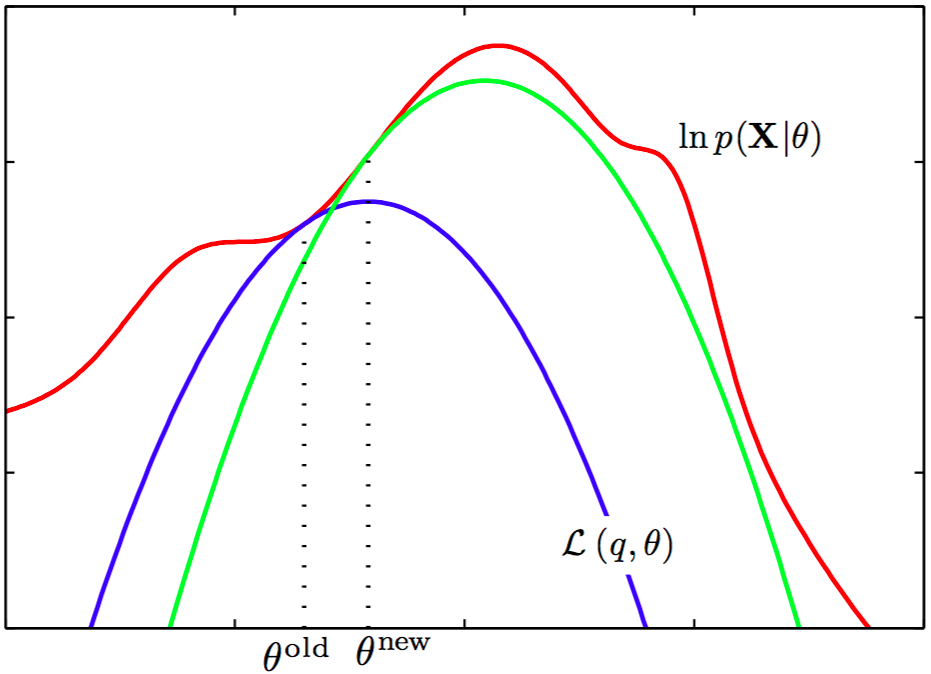
\includegraphics[height=5cm]{figures/EM-twosteps-Bishop9.14.png}
    \end{figure}
    \vspace{-2em}
    Exercise: prove that EM increases the marginal likelihood monotonically
    $$
    \log p(x;\theta^{\text{new}}) \ge \log p(x;\theta^{\text{old}})
    \;.
    $$
    Does EM converge to a global maximum?
\end{frame}

\begin{frame}
    {EM for multinomial naive Bayes}
    \emph{Setting}: $x = (x_1,\ldots,x_m) \in \sV^m, z\in\pc{1,\ldots,K}, \sD=\pc{x^{(i)}}_{i=1}^N$

    \emph{E-step}:
    \vspace{-1em}
    \begin{align*}
        &q^*(z) = p(z\mid x; \theta^{\text{old}}) = 
        \frac{\prod_{i=1}^m p(x_i\mid z; \theta^{\text{old}})p(z;\theta^{\text{old}})}
        {\sum_{z'\in\sZ} \prod_{i=1}^m p(x_i\mid z'; \theta^{\text{old}})p(z';\theta^{\text{old}})}\\
        &J(\theta) = \sum_{{\color{blue}x}\in\sD} \sum_{z\in\sZ} q^*_{\color{blue}x}(z) {\log p(x,z;\theta)} 
        = \sum_{x\in\sD} \sum_{z\in\sZ} q^*_x(z) \log
        {\prod_{i=1}^m p(x_i\mid z;\theta) p(z;\theta)} 
    \end{align*}

    \emph{M-step}:
    \vspace{-1em}
    \begin{align*}
        \max_\theta& \sum_{x\in\sD} \sum_{z\in\sZ}q^*_x(z)\p{ \sum_{w\in\sV}
        \log \theta_{w\mid z}^{\text{count}(w\mid x)} + \log \theta_z }\\
        \text{s.t.} & \quad \sum_{w\in\sV} \theta_{w\mid z} = 1 \quad \forall w\in\sV,
        \quad \sum_{z\in\sZ}\theta_z = 1 \;,\\
        \text{where } & \text{count}(w\mid x) \eqdef \text{\# occurrence of $w$ in $x$}
    \end{align*}
\end{frame}

\begin{frame}
    {EM for multinomial naive Bayes}
    M-step has closed-form solution:
    \begin{align*}
        \theta_z &= \frac{\sum_{x\in\sD} q^*_x(z)}
        {\sum_{z\in\sZ} \sum_{x\in\sD}\underbrace{q^*_x(z)}_{\text{soft label count}}}\\
        \theta_{w\mid z} &= \frac{
            \sum_{x\in\sD} q^*_x(z)\text{count}(w\mid x)  
        }{
            \sum_{w\in\sV}\sum_{x\in\sD} \underbrace{q^*_x(z)\text{count}(w\mid x)}_{\text{soft word count}
        }}
    \end{align*}
    Similar to the MLE solution except that we're using soft counts.
\end{frame}

\begin{frame}
    {M-step for multinomial naive Bayes}
    \begin{align*}
        \max_\theta& \sum_{x\in\sD} \sum_{z\in\sZ}q^*_x(z)\p{ \sum_{w\in\sV}
        \log \theta_{w\mid z}^{\text{count}(w\mid x)} + \log \theta_z }\\
        \text{s.t.} & \quad \sum_{w\in\sV} \theta_{w\mid z} = 1 \quad \forall w\in\sV,
        \quad \sum_{z\in\sZ}\theta_z = 1
    \end{align*}
    \vspace{14em}
\end{frame}

\begin{frame}
    {Summary}
    \textbf{Expectation minimization (EM)} algorithm:
    maximizing ELBO $\sL(q, \theta)$ by coordinate ascent

    \textbf{E-step}:
    Compute the expected complete data log-likelihood $J(\theta)$
    using
    $q^*(z) = p(z\mid x; \theta^{\text{old}})$

    \textbf{M-step}:
        Maximize $J(\theta)$ to obtain $\theta^{\text{new}}$
        
    \emph{Assumptions:}
    E-step and M-step are easy to compute

    \emph{Properties}:
        Monotonically improve the likelihood and converge to a stationary point
\end{frame}

\section{EM for HMM}

\begin{frame}
    {HMM recap}
    Setting:\\
    \begin{itemize}
        \item Hidden states $z_i \in \sY$ (e.g. POS tags)
        \item Observations $x_i\in \sX$ (e.g. words)
    \end{itemize}
    $$
    p(x_{1:m},y_{1:m}) = \prod_{i=1}^m \underbrace{p(x_i\mid y_i)}_{\text{emission probability}}
    \prod_{i=1}^m \underbrace{p(y_i\mid y_{i-1})}_{\text{transition probability}}
    $$
    Parameters:\\
    \begin{itemize}
        \item Transition probabilities: $p(y_i=t\mid y_{i-1}=t') = \theta_{t\mid t'}$
        \item Emission probabilities: $p(x_i=w\mid y_i=t) = \gamma_{w\mid t}$
        \item $y_0=*, y_m=\texttt{STOP}$
    \end{itemize}
    Task: estimate parameters given \emph{incomplete} observations
\end{frame}

\begin{frame}
    {E-step for HMM}
    E-step: 
    \begin{align*}
        q^*(z) &= p(z\mid x; \theta, \gamma) \\
        \sL(q^*, \theta, \gamma) &= \sum_{x\in\sD} \underbrace{\sum_{z\in\sZ} q^*_x(z)
        \log p(x,z;\theta,\gamma)}_\text{expected complete log-likelihood} \\
        &= \sum_{x\in\sD} \sum_{z\in\sZ} q^*_x(z)
        \log \underbrace{\prod_{i=1}^m p(x_i\mid z_i) p(z_i\mid z_{i-1})}_{\text{HMM}} \\
        &= \sum_{x\in\sD} \sum_{z\in\sZ} q^*_x(z)
        \sum_{i=1}^m \p{
            \log \underbrace{p(x_i\mid z_i; \gamma)}_{\gamma_{x_i\mid z_i}} + 
        \log \underbrace{p(z_i\mid z_{i-1}; \theta)}_{\theta_{z_i\mid z_{i-1}}} 
        }
    \end{align*}
\end{frame}

\begin{frame}
    {M-step for HMM}
    M-step (similar to the NB solution):
    \begin{align*}
        \max_{\theta,\gamma} \sL(q^*, \theta, \gamma) = \sum_{x\in\sD} \sum_{z\in\sZ} q^*_x(z)
        \sum_{i=1}^m \p{ \log\gamma_{x_i\mid z_i} + \log \theta_{z_i\mid z_{i-1}} }
    \end{align*}
    Emission probabilities:
    \begin{align*}
        \gamma_{w\mid t} &= \frac{
            \sum_{x\in\sD} \sum_{z\in\sZ} q^*_x(z) \text{count}(w,t\mid x,z)
        }{
            \sum_{w'\in\sX} \sum_{x\in\sD} \sum_{z\in\sZ} q^*_x(z) \text{count}(w',t\mid x,z)
        }\\
        \text{count}(w,t\mid x,z) &\eqdef \text{\# word-tag pairs $(w,t)$ in $(x,z)$} 
    \end{align*}
    Transition probabilities:
    \begin{align*}
        \theta_{t\mid t'} &= \frac{
            \sum_{x\in\sD} \sum_{z\in\sZ} q^*_x(z) \text{count}(t'\rightarrow t\mid z)
        }{
            \sum_{a\in\sY} \sum_{x\in\sD} \sum_{z\in\sZ} q^*_x(z) \text{count}(t'\rightarrow a\mid z)
        }\\
        \text{count}(t'\rightarrow t\mid z) &\eqdef \text{\# tag bigrams $(t',t)$ in $z$} 
    \end{align*}
\end{frame}

\begin{frame}
    {M-step for HMM}
    \emph{Challenge}: $\sum_{{\color{blue}z\in\sY^m}} q^*_x(z) \text{count}(w,t\mid x,z)$

    \vspace{5em}
    
    \begin{center}
    \begin{tikzpicture}
        \foreach \i\j\k in {0/the/DT, 1/fox/NN, 2/jumped/VBD, 3/over/IN, 4/the/DT, 5/dog/NN}{
            \node[anchor=base] (i\i) at (1.5*\i, 0) {\j};
            \node[anchor=base] (o\i) at (1.5*\i, 1) {\k};
            \path[draw,arrow,blue] (o\i.south) -- (i\i.north);
        }
        \foreach \i in {1,...,5}{
            \pgfmathtruncatemacro\j{\i-1}
            \path[draw,arrow,red] (o\j.east) -- (o\i.west);
        }
    \end{tikzpicture}
    \end{center}
    Group sequences where $z_i=t$:
    \begin{align*}
    \sum_{{z\in\sY^m}} q^*_x(z) \text{count}(w,t\mid x,z)
        &= \sum_{i=1}^m \mu_x(z_i=t) \1\pb{x_i=w} \\
        \mu_x(z_i=t) &= \sum_{\pc{z\in\sY^m \mid z_i=t}} q^*_x(z)
    \end{align*}
\end{frame}

\begin{frame}
    {M-step for HMM}
    \emph{Challenge}: $\sum_{{\color{blue}z\in\sY^m}} q^*_x(z) \text{count}(t'\rightarrow t\mid z)$

    \vspace{5em}
    
    \begin{center}
    \begin{tikzpicture}
        \foreach \i\j\k in {0/the/DT, 1/fox/NN, 2/jumped/VBD, 3/over/IN, 4/the/DT, 5/dog/NN}{
            \node[anchor=base] (i\i) at (1.5*\i, 0) {\j};
            \node[anchor=base] (o\i) at (1.5*\i, 1) {\k};
            \path[draw,arrow,blue] (o\i.south) -- (i\i.north);
        }
        \foreach \i in {1,...,5}{
            \pgfmathtruncatemacro\j{\i-1}
            \path[draw,arrow,red] (o\j.east) -- (o\i.west);
        }
    \end{tikzpicture}
    \end{center}
    Group sequences where $z_i=t, z_{i-1}=t'$:
    \begin{align*}
    \sum_{{z\in\sY^m}} q^*_x(z) \text{count}(t'\rightarrow t\mid z)
        &= \sum_{i=1}^m \mu_x(z_i=t,z_{i-1}=t')  \\
        \mu_x(z_i=t) &= \sum_{\pc{z\in\sY^m \mid z_i=t, z_{i-1}=t}} q^*_x(z)
    \end{align*}
\end{frame}

\begin{frame}
    {Compute tag marginals}
    $\mu_x(z_i=t)$: probability of the $i$-th tag being $t$ given observed words $x$
    \begin{align*}
        \mu_x(z_i=t) &= \sum_{z: z_i=t} q^*_x(z) \;
        {\color{red}\propto} \sum_{z: z_i=t} \prod_{j=1}^m \underbrace{q(x_i\mid z_i) q(z_i\mid z_{i-1})}_{\psi(z_i,z_{i-1})} \\
        &= \sum_{z: z_i=t} \prod_{j=1}^{i-1}\psi(z_j,z_{j-1})\prod_{j=i}^m\psi(z_j,z_{j-1}) \\
        &= \sum_{t'} \sum_{z: z_i=t,z_{i-1}=t'} \prod_{j=1}^{i-1}\psi(z_j,z_{j-1})\prod_{j=i}^m\psi(z_j,z_{j-1}) \\
        &= \sum_{t'} \p{
            \sum_{\substack{z_{1:i-1}\\z_{i-1}=t'}}  \prod_{j=1}^{i-1}\psi(z_j,z_{j-1})
        }
        \psi(t,t')
        \p{\sum_{\substack{z_{i+1:m}\\z_i=t}} \prod_{j=i}^{m}\psi(z_j,z_{j-1})
        } \\
        &= \sum_{t'} \alpha[i-1, t] \psi(t,t') \beta[i, t]
        = {\color{blue}\alpha[i,t] \beta[i,t]}
    \end{align*}
\end{frame}

\begin{frame}
    {Compute tag marginals}
    \textbf{Forward probabilities}: probability of tag sequence prefix ending at $z_i=t$.
    \begin{align*}
        \alpha[i,t] &\eqdef q(x_1,\ldots,x_i,z_i=t) \\
        \alpha[i,t] &= \sum_{t'\in\sY} \alpha[i-1,t']\psi(t',t)
    \end{align*}

    \textbf{Backward probabilities}: probability of tag sequence suffix starting from $z_{i+1}$ give $z_i=t$.
    \begin{align*}
        \beta[i,t] &\eqdef q(x_{i+1},\ldots,x_m\mid z_i=t) \\
        \beta[i,t] &= \sum_{t'\in\sY} \beta[i+1,t']\psi(t,t')
    \end{align*}
\end{frame}

\begin{frame}
    {Compute tag marginals}
    \begin{enumerate}
        \item Compute forward and backward probabilities
            \begin{align*}
                \alpha[i,t] &\quad \forall i\in\pc{1,\ldots,m}, t\in\sY\cup\pc{\texttt{STOP}}\\
                \beta[i,t] &\quad \forall i\in\pc{m,\dots,1}, t\in\sY\cup\pc{*}
            \end{align*}
        \item Comptute the tag unigram and bigram marginals
    \begin{align*}
        \mu_x(z_i=t) &\eqdef q(z_i=t\mid x) \\
        &= \frac{\alpha[i,t]\beta[i,t]}{q(x)}
        = \frac{\alpha[i,t]\beta[i,t]}{\alpha[m,\texttt{STOP}]} \\
        \mu_x(z_{i-1}=t',z_i=t) &\eqdef q(z_{i-1}=t',z_i=t\mid x) \\
        &= \frac{\alpha[i-1,t']\psi(t',t)\beta[i,t]}{q(x)}
    \end{align*}
    \end{enumerate}
    In practice, compute in the \emph{log space}.
\end{frame}

\begin{frame}
    {Updated parameters}
    Emission probabilities:
    \begin{align*}
        \gamma_{w\mid t} &= \frac{
            \sum_{x\in\sD} \sum_{z\in\sZ} q^*_x(z) \text{count}(w,t\mid x,z)
        }{
            \sum_{w'\in\sX} \sum_{x\in\sD} \sum_{z\in\sZ} q^*_x(z) \text{count}(w',t\mid x,z)
        }\\
        &= \frac{
            \sum_{x\in\sD} \sum_{i=1}^m \mu_x(z_i=t) \1\pb{x_i=w}
        }{
            \sum_{w'\in\sX} \sum_{x\in\sD} \sum_{i=1}^m \mu_x(z_i=t) \1\pb{x_i=w'}
        }
    \end{align*}
    Transition probabilities:
    \begin{align*}
        \theta_{t\mid t'} &= \frac{
            \sum_{x\in\sD} \sum_{z\in\sZ} q^*_x(z) \text{count}(t'\rightarrow t\mid z)
        }{
            \sum_{a\in\sY} \sum_{x\in\sD} \sum_{z\in\sZ} q^*_x(z) \text{count}(t'\rightarrow a\mid z)
        }\\
        &= \frac{
            \sum_{x\in\sD}\sum_{i=1}^m \mu_x(z_{i-1}=t',z_i=t)
        }{
            \sum_{a\in\sY} \sum_{x\in\sD}\sum_{i=1}^m \mu_x(z_{i-1}=t',z_i=a)
        }
    \end{align*}
\end{frame}

\begin{frame}
    {Summary}
    EM for HMM:\\
    \begin{enumerate}
        \item Randomly initialize the emission and transition probabilities
        \item Repeat until convergence
            \begin{enumerate}[(i)]
                \item Compute forward and backward probabilities
                \item Update the emission and transition probabilities using expected counts
            \end{enumerate}
        \item[] If the solution is bad, re-run EM with a different random seed.
    \end{enumerate}

    General EM:\\
    \begin{itemize}
        \item One example of variational methods (use a tractable $q$ to approximate $p$)
        \item May need approximation in both the E-step and the M-step
        \item Useful in probabilistic models and Bayesian methods
    \end{itemize}
\end{frame}

\end{document}
